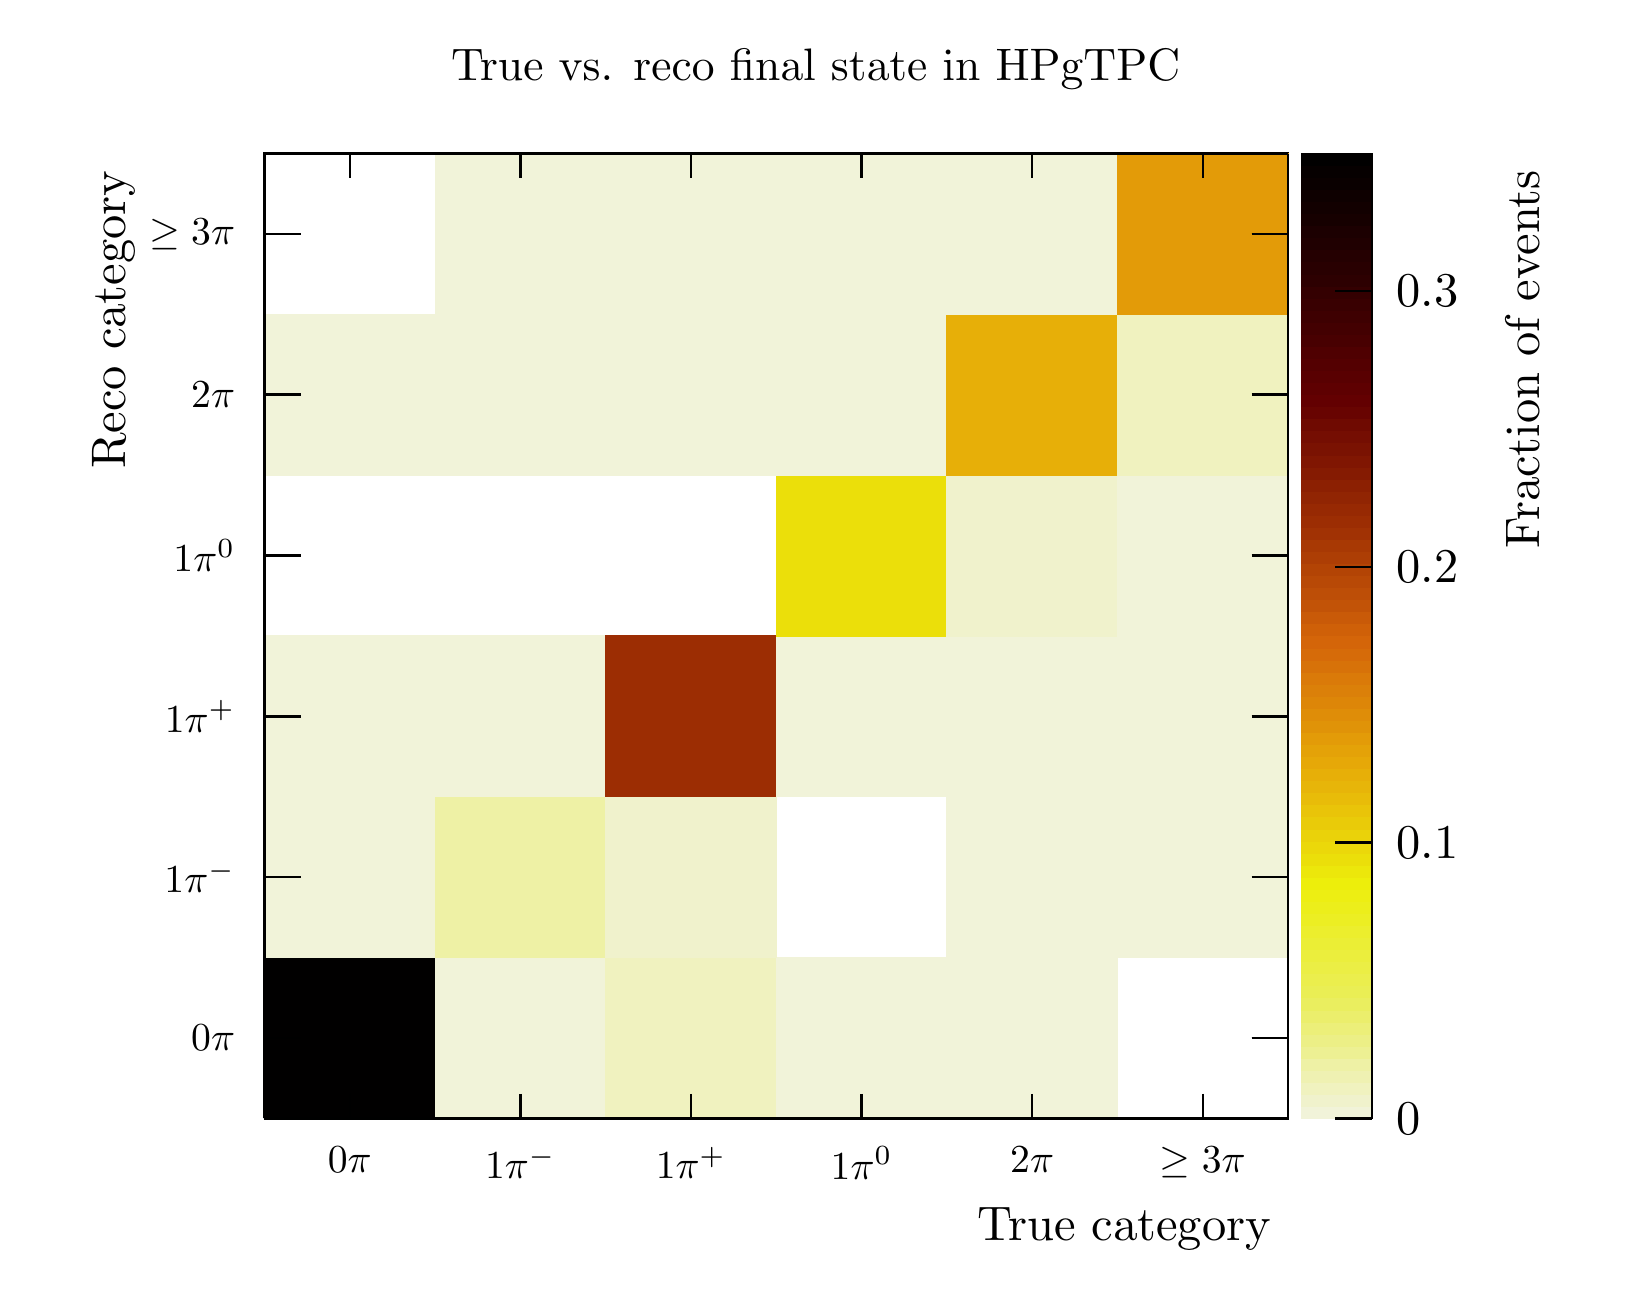
\begin{tikzpicture}
\pgfdeclareplotmark{cross} {
\pgfpathmoveto{\pgfpoint{-0.3\pgfplotmarksize}{\pgfplotmarksize}}
\pgfpathlineto{\pgfpoint{+0.3\pgfplotmarksize}{\pgfplotmarksize}}
\pgfpathlineto{\pgfpoint{+0.3\pgfplotmarksize}{0.3\pgfplotmarksize}}
\pgfpathlineto{\pgfpoint{+1\pgfplotmarksize}{0.3\pgfplotmarksize}}
\pgfpathlineto{\pgfpoint{+1\pgfplotmarksize}{-0.3\pgfplotmarksize}}
\pgfpathlineto{\pgfpoint{+0.3\pgfplotmarksize}{-0.3\pgfplotmarksize}}
\pgfpathlineto{\pgfpoint{+0.3\pgfplotmarksize}{-1.\pgfplotmarksize}}
\pgfpathlineto{\pgfpoint{-0.3\pgfplotmarksize}{-1.\pgfplotmarksize}}
\pgfpathlineto{\pgfpoint{-0.3\pgfplotmarksize}{-0.3\pgfplotmarksize}}
\pgfpathlineto{\pgfpoint{-1.\pgfplotmarksize}{-0.3\pgfplotmarksize}}
\pgfpathlineto{\pgfpoint{-1.\pgfplotmarksize}{0.3\pgfplotmarksize}}
\pgfpathlineto{\pgfpoint{-0.3\pgfplotmarksize}{0.3\pgfplotmarksize}}
\pgfpathclose
\pgfusepathqstroke
}
\pgfdeclareplotmark{cross*} {
\pgfpathmoveto{\pgfpoint{-0.3\pgfplotmarksize}{\pgfplotmarksize}}
\pgfpathlineto{\pgfpoint{+0.3\pgfplotmarksize}{\pgfplotmarksize}}
\pgfpathlineto{\pgfpoint{+0.3\pgfplotmarksize}{0.3\pgfplotmarksize}}
\pgfpathlineto{\pgfpoint{+1\pgfplotmarksize}{0.3\pgfplotmarksize}}
\pgfpathlineto{\pgfpoint{+1\pgfplotmarksize}{-0.3\pgfplotmarksize}}
\pgfpathlineto{\pgfpoint{+0.3\pgfplotmarksize}{-0.3\pgfplotmarksize}}
\pgfpathlineto{\pgfpoint{+0.3\pgfplotmarksize}{-1.\pgfplotmarksize}}
\pgfpathlineto{\pgfpoint{-0.3\pgfplotmarksize}{-1.\pgfplotmarksize}}
\pgfpathlineto{\pgfpoint{-0.3\pgfplotmarksize}{-0.3\pgfplotmarksize}}
\pgfpathlineto{\pgfpoint{-1.\pgfplotmarksize}{-0.3\pgfplotmarksize}}
\pgfpathlineto{\pgfpoint{-1.\pgfplotmarksize}{0.3\pgfplotmarksize}}
\pgfpathlineto{\pgfpoint{-0.3\pgfplotmarksize}{0.3\pgfplotmarksize}}
\pgfpathclose
\pgfusepathqfillstroke
}
\pgfdeclareplotmark{newstar} {
\pgfpathmoveto{\pgfqpoint{0pt}{\pgfplotmarksize}}
\pgfpathlineto{\pgfqpointpolar{44}{0.5\pgfplotmarksize}}
\pgfpathlineto{\pgfqpointpolar{18}{\pgfplotmarksize}}
\pgfpathlineto{\pgfqpointpolar{-20}{0.5\pgfplotmarksize}}
\pgfpathlineto{\pgfqpointpolar{-54}{\pgfplotmarksize}}
\pgfpathlineto{\pgfqpointpolar{-90}{0.5\pgfplotmarksize}}
\pgfpathlineto{\pgfqpointpolar{234}{\pgfplotmarksize}}
\pgfpathlineto{\pgfqpointpolar{198}{0.5\pgfplotmarksize}}
\pgfpathlineto{\pgfqpointpolar{162}{\pgfplotmarksize}}
\pgfpathlineto{\pgfqpointpolar{134}{0.5\pgfplotmarksize}}
\pgfpathclose
\pgfusepathqstroke
}
\pgfdeclareplotmark{newstar*} {
\pgfpathmoveto{\pgfqpoint{0pt}{\pgfplotmarksize}}
\pgfpathlineto{\pgfqpointpolar{44}{0.5\pgfplotmarksize}}
\pgfpathlineto{\pgfqpointpolar{18}{\pgfplotmarksize}}
\pgfpathlineto{\pgfqpointpolar{-20}{0.5\pgfplotmarksize}}
\pgfpathlineto{\pgfqpointpolar{-54}{\pgfplotmarksize}}
\pgfpathlineto{\pgfqpointpolar{-90}{0.5\pgfplotmarksize}}
\pgfpathlineto{\pgfqpointpolar{234}{\pgfplotmarksize}}
\pgfpathlineto{\pgfqpointpolar{198}{0.5\pgfplotmarksize}}
\pgfpathlineto{\pgfqpointpolar{162}{\pgfplotmarksize}}
\pgfpathlineto{\pgfqpointpolar{134}{0.5\pgfplotmarksize}}
\pgfpathclose
\pgfusepathqfillstroke
}
\definecolor{c}{rgb}{1,1,1};
\draw [color=c, fill=c] (0,0) rectangle (20,15.914);
\draw [color=c, fill=c] (3,2.06882) rectangle (16,14.3226);
\definecolor{c}{rgb}{0,0,0};
\draw [c,line width=0.9] (3,2.06882) -- (3,14.3226) -- (16,14.3226) -- (16,2.06882) -- (3,2.06882);
\definecolor{c}{rgb}{1,1,1};
\draw [color=c, fill=c] (3,2.06882) rectangle (16,14.3226);
\definecolor{c}{rgb}{0,0,0};
\draw [c,line width=0.9] (3,2.06882) -- (3,14.3226) -- (16,14.3226) -- (16,2.06882) -- (3,2.06882);
\definecolor{c}{rgb}{0.00551471,0,0.000122549};
\draw [color=c, fill=c] (3,2.06882) rectangle (5.16667,4.11111);
\definecolor{c}{rgb}{0.945984,0.951044,0.850727};
\draw [color=c, fill=c] (5.16667,2.06882) rectangle (7.33333,4.11111);
\definecolor{c}{rgb}{0.939911,0.947249,0.748261};
\draw [color=c, fill=c] (7.33333,2.06882) rectangle (9.5,4.11111);
\definecolor{c}{rgb}{0.945984,0.951044,0.850727};
\draw [color=c, fill=c] (9.5,2.06882) rectangle (11.6667,4.11111);
\draw [color=c, fill=c] (11.6667,2.06882) rectangle (13.8333,4.11111);
\draw [color=c, fill=c] (3,4.11111) rectangle (5.16667,6.15341);
\definecolor{c}{rgb}{0.933839,0.943453,0.645794};
\draw [color=c, fill=c] (5.16667,4.11111) rectangle (7.33333,6.15341);
\definecolor{c}{rgb}{0.942948,0.949146,0.799494};
\draw [color=c, fill=c] (7.33333,4.11111) rectangle (9.5,6.15341);
\definecolor{c}{rgb}{0.945984,0.951044,0.850727};
\draw [color=c, fill=c] (11.6667,4.11111) rectangle (13.8333,6.15341);
\draw [color=c, fill=c] (13.8333,4.11111) rectangle (16,6.15341);
\draw [color=c, fill=c] (3,6.15341) rectangle (5.16667,8.1957);
\draw [color=c, fill=c] (5.16667,6.15341) rectangle (7.33333,8.1957);
\definecolor{c}{rgb}{0.611765,0.176471,0.0117647};
\draw [color=c, fill=c] (7.33333,6.15341) rectangle (9.5,8.1957);
\definecolor{c}{rgb}{0.945984,0.951044,0.850727};
\draw [color=c, fill=c] (9.5,6.15341) rectangle (11.6667,8.1957);
\draw [color=c, fill=c] (11.6667,6.15341) rectangle (13.8333,8.1957);
\draw [color=c, fill=c] (13.8333,6.15341) rectangle (16,8.1957);
\definecolor{c}{rgb}{0.923407,0.873284,0.0405637};
\draw [color=c, fill=c] (9.5,8.1957) rectangle (11.6667,10.238);
\definecolor{c}{rgb}{0.942948,0.949146,0.799494};
\draw [color=c, fill=c] (11.6667,8.1957) rectangle (13.8333,10.238);
\definecolor{c}{rgb}{0.945984,0.951044,0.850727};
\draw [color=c, fill=c] (13.8333,8.1957) rectangle (16,10.238);
\draw [color=c, fill=c] (3,10.238) rectangle (5.16667,12.2803);
\draw [color=c, fill=c] (5.16667,10.238) rectangle (7.33333,12.2803);
\draw [color=c, fill=c] (7.33333,10.238) rectangle (9.5,12.2803);
\draw [color=c, fill=c] (9.5,10.238) rectangle (11.6667,12.2803);
\definecolor{c}{rgb}{0.904534,0.684559,0.0324755};
\draw [color=c, fill=c] (11.6667,10.238) rectangle (13.8333,12.2803);
\definecolor{c}{rgb}{0.939911,0.947249,0.748261};
\draw [color=c, fill=c] (13.8333,10.238) rectangle (16,12.2803);
\definecolor{c}{rgb}{0.945984,0.951044,0.850727};
\draw [color=c, fill=c] (5.16667,12.2803) rectangle (7.33333,14.3226);
\draw [color=c, fill=c] (7.33333,12.2803) rectangle (9.5,14.3226);
\draw [color=c, fill=c] (9.5,12.2803) rectangle (11.6667,14.3226);
\draw [color=c, fill=c] (11.6667,12.2803) rectangle (13.8333,14.3226);
\definecolor{c}{rgb}{0.888726,0.609559,0.0321078};
\draw [color=c, fill=c] (13.8333,12.2803) rectangle (16,14.3226);
\definecolor{c}{rgb}{0,0,0};
\draw [c,line width=0.9] (3,2.06882) -- (16,2.06882);
\draw [anchor=north] (4.08333,1.88501) node[scale=1.43288, color=c, rotate=0]{$0\pi$};
\draw [anchor=north] (6.25,1.88501) node[scale=1.43288, color=c, rotate=0]{$1\pi^{-}$};
\draw [anchor=north] (8.41667,1.88501) node[scale=1.43288, color=c, rotate=0]{$1\pi^{+}$};
\draw [anchor=north] (10.5833,1.88501) node[scale=1.43288, color=c, rotate=0]{$1\pi^{0}$};
\draw [anchor=north] (12.75,1.88501) node[scale=1.43288, color=c, rotate=0]{$2\pi$};
\draw [anchor=north] (14.9167,1.88501) node[scale=1.43288, color=c, rotate=0]{$\geq3\pi$};
\draw [c,line width=0.9] (4.08333,2.37914) -- (4.08333,2.06882);
\draw [c,line width=0.9] (6.25,2.37914) -- (6.25,2.06882);
\draw [c,line width=0.9] (8.41667,2.37914) -- (8.41667,2.06882);
\draw [c,line width=0.9] (10.5833,2.37914) -- (10.5833,2.06882);
\draw [c,line width=0.9] (12.75,2.37914) -- (12.75,2.06882);
\draw [c,line width=0.9] (14.9167,2.37914) -- (14.9167,2.06882);
\draw [c,line width=0.9] (4.08333,2.37914) -- (4.08333,2.06882);
\draw [c,line width=0.9] (14.9167,2.37914) -- (14.9167,2.06882);
\draw [anchor= east] (16,0.668387) node[scale=1.7513, color=c, rotate=0]{ True category};
\draw [c,line width=0.9] (3,14.3226) -- (16,14.3226);
\draw [c,line width=0.9] (4.08333,14.0123) -- (4.08333,14.3226);
\draw [c,line width=0.9] (6.25,14.0123) -- (6.25,14.3226);
\draw [c,line width=0.9] (8.41667,14.0123) -- (8.41667,14.3226);
\draw [c,line width=0.9] (10.5833,14.0123) -- (10.5833,14.3226);
\draw [c,line width=0.9] (12.75,14.0123) -- (12.75,14.3226);
\draw [c,line width=0.9] (14.9167,14.0123) -- (14.9167,14.3226);
\draw [c,line width=0.9] (4.08333,14.0123) -- (4.08333,14.3226);
\draw [c,line width=0.9] (14.9167,14.0123) -- (14.9167,14.3226);
\draw [c,line width=0.9] (3,2.06882) -- (3,14.3226);
\draw [anchor= east] (2.805,3.08996) node[scale=1.43288, color=c, rotate=0]{$0\pi$};
\draw [anchor= east] (2.805,5.13226) node[scale=1.43288, color=c, rotate=0]{$1\pi^{-}$};
\draw [anchor= east] (2.805,7.17455) node[scale=1.43288, color=c, rotate=0]{$1\pi^{+}$};
\draw [anchor= east] (2.805,9.21685) node[scale=1.43288, color=c, rotate=0]{$1\pi^{0}$};
\draw [anchor= east] (2.805,11.2591) node[scale=1.43288, color=c, rotate=0]{$2\pi$};
\draw [anchor= east] (2.805,13.3014) node[scale=1.43288, color=c, rotate=0]{$\geq3\pi$};
\draw [c,line width=0.9] (3.462,3.08996) -- (3,3.08996);
\draw [c,line width=0.9] (3.462,5.13226) -- (3,5.13226);
\draw [c,line width=0.9] (3.462,7.17455) -- (3,7.17455);
\draw [c,line width=0.9] (3.462,9.21685) -- (3,9.21685);
\draw [c,line width=0.9] (3.462,11.2591) -- (3,11.2591);
\draw [c,line width=0.9] (3.462,13.3014) -- (3,13.3014);
\draw [c,line width=0.9] (3.462,3.08996) -- (3,3.08996);
\draw [c,line width=0.9] (3.462,13.3014) -- (3,13.3014);
\draw [anchor= east] (1.08,14.3226) node[scale=1.7513, color=c, rotate=90]{ Reco category};
\draw [c,line width=0.9] (16,2.06882) -- (16,14.3226);
\draw [c,line width=0.9] (15.538,3.08996) -- (16,3.08996);
\draw [c,line width=0.9] (15.538,5.13226) -- (16,5.13226);
\draw [c,line width=0.9] (15.538,7.17455) -- (16,7.17455);
\draw [c,line width=0.9] (15.538,9.21685) -- (16,9.21685);
\draw [c,line width=0.9] (15.538,11.2591) -- (16,11.2591);
\draw [c,line width=0.9] (15.538,13.3014) -- (16,13.3014);
\draw [c,line width=0.9] (15.538,3.08996) -- (16,3.08996);
\draw [c,line width=0.9] (15.538,13.3014) -- (16,13.3014);
\definecolor{c}{rgb}{0.945984,0.951044,0.850727};
\draw [color=c, fill=c] (16.1686,2.06691) rectangle (17.0626,2.22013);
\definecolor{c}{rgb}{0.942948,0.949146,0.799494};
\draw [color=c, fill=c] (16.1686,2.22013) rectangle (17.0626,2.37336);
\definecolor{c}{rgb}{0.939911,0.947249,0.748261};
\draw [color=c, fill=c] (16.1686,2.37336) rectangle (17.0626,2.52658);
\definecolor{c}{rgb}{0.936875,0.945351,0.697027};
\draw [color=c, fill=c] (16.1686,2.52658) rectangle (17.0626,2.67981);
\definecolor{c}{rgb}{0.933839,0.943453,0.645794};
\draw [color=c, fill=c] (16.1686,2.67981) rectangle (17.0626,2.83303);
\definecolor{c}{rgb}{0.929791,0.940923,0.577483};
\draw [color=c, fill=c] (16.1686,2.83303) rectangle (17.0626,2.98626);
\definecolor{c}{rgb}{0.926755,0.939026,0.526249};
\draw [color=c, fill=c] (16.1686,2.98626) rectangle (17.0626,3.13949);
\definecolor{c}{rgb}{0.923719,0.937128,0.475016};
\draw [color=c, fill=c] (16.1686,3.13949) rectangle (17.0626,3.29271);
\definecolor{c}{rgb}{0.920683,0.935231,0.423782};
\draw [color=c, fill=c] (16.1686,3.29271) rectangle (17.0626,3.44594);
\definecolor{c}{rgb}{0.917647,0.933333,0.372549};
\draw [color=c, fill=c] (16.1686,3.44594) rectangle (17.0626,3.59916);
\definecolor{c}{rgb}{0.919118,0.933333,0.331373};
\draw [color=c, fill=c] (16.1686,3.59916) rectangle (17.0626,3.75239);
\definecolor{c}{rgb}{0.920221,0.933333,0.30049};
\draw [color=c, fill=c] (16.1686,3.75239) rectangle (17.0626,3.90562);
\definecolor{c}{rgb}{0.921324,0.933333,0.269608};
\draw [color=c, fill=c] (16.1686,3.90562) rectangle (17.0626,4.05884);
\definecolor{c}{rgb}{0.922426,0.933333,0.238725};
\draw [color=c, fill=c] (16.1686,4.05884) rectangle (17.0626,4.21207);
\definecolor{c}{rgb}{0.923529,0.933333,0.207843};
\draw [color=c, fill=c] (16.1686,4.21207) rectangle (17.0626,4.36529);
\definecolor{c}{rgb}{0.924632,0.933333,0.176961};
\draw [color=c, fill=c] (16.1686,4.36529) rectangle (17.0626,4.51852);
\definecolor{c}{rgb}{0.926103,0.933333,0.135784};
\draw [color=c, fill=c] (16.1686,4.51852) rectangle (17.0626,4.67174);
\definecolor{c}{rgb}{0.927206,0.933333,0.104902};
\draw [color=c, fill=c] (16.1686,4.67174) rectangle (17.0626,4.82497);
\definecolor{c}{rgb}{0.928309,0.933333,0.0740196};
\draw [color=c, fill=c] (16.1686,4.82497) rectangle (17.0626,4.9782);
\definecolor{c}{rgb}{0.929412,0.933333,0.0431373};
\draw [color=c, fill=c] (16.1686,4.9782) rectangle (17.0626,5.13142);
\definecolor{c}{rgb}{0.926838,0.907598,0.0420343};
\draw [color=c, fill=c] (16.1686,5.13142) rectangle (17.0626,5.28465);
\definecolor{c}{rgb}{0.923407,0.873284,0.0405637};
\draw [color=c, fill=c] (16.1686,5.28465) rectangle (17.0626,5.43787);
\definecolor{c}{rgb}{0.920833,0.847549,0.0394608};
\draw [color=c, fill=c] (16.1686,5.43787) rectangle (17.0626,5.5911);
\definecolor{c}{rgb}{0.91826,0.821814,0.0383578};
\draw [color=c, fill=c] (16.1686,5.5911) rectangle (17.0626,5.74433);
\definecolor{c}{rgb}{0.915686,0.796078,0.0372549};
\draw [color=c, fill=c] (16.1686,5.74433) rectangle (17.0626,5.89755);
\definecolor{c}{rgb}{0.913113,0.770343,0.036152};
\draw [color=c, fill=c] (16.1686,5.89755) rectangle (17.0626,6.05078);
\definecolor{c}{rgb}{0.909681,0.736029,0.0346814};
\draw [color=c, fill=c] (16.1686,6.05078) rectangle (17.0626,6.204);
\definecolor{c}{rgb}{0.907108,0.710294,0.0335784};
\draw [color=c, fill=c] (16.1686,6.204) rectangle (17.0626,6.35723);
\definecolor{c}{rgb}{0.904534,0.684559,0.0324755};
\draw [color=c, fill=c] (16.1686,6.35723) rectangle (17.0626,6.51045);
\definecolor{c}{rgb}{0.901961,0.658824,0.0313726};
\draw [color=c, fill=c] (16.1686,6.51045) rectangle (17.0626,6.66368);
\definecolor{c}{rgb}{0.895343,0.634191,0.0317402};
\draw [color=c, fill=c] (16.1686,6.66368) rectangle (17.0626,6.81691);
\definecolor{c}{rgb}{0.888726,0.609559,0.0321078};
\draw [color=c, fill=c] (16.1686,6.81691) rectangle (17.0626,6.97013);
\definecolor{c}{rgb}{0.879902,0.576716,0.032598};
\draw [color=c, fill=c] (16.1686,6.97013) rectangle (17.0626,7.12336);
\definecolor{c}{rgb}{0.873284,0.552083,0.0329657};
\draw [color=c, fill=c] (16.1686,7.12336) rectangle (17.0626,7.27658);
\definecolor{c}{rgb}{0.866667,0.527451,0.0333333};
\draw [color=c, fill=c] (16.1686,7.27658) rectangle (17.0626,7.42981);
\definecolor{c}{rgb}{0.860049,0.502819,0.033701};
\draw [color=c, fill=c] (16.1686,7.42981) rectangle (17.0626,7.58303);
\definecolor{c}{rgb}{0.853431,0.478186,0.0340686};
\draw [color=c, fill=c] (16.1686,7.58303) rectangle (17.0626,7.73626);
\definecolor{c}{rgb}{0.844608,0.445343,0.0345588};
\draw [color=c, fill=c] (16.1686,7.73626) rectangle (17.0626,7.88949);
\definecolor{c}{rgb}{0.83799,0.420711,0.0349265};
\draw [color=c, fill=c] (16.1686,7.88949) rectangle (17.0626,8.04271);
\definecolor{c}{rgb}{0.831373,0.396078,0.0352941};
\draw [color=c, fill=c] (16.1686,8.04271) rectangle (17.0626,8.19594);
\definecolor{c}{rgb}{0.810784,0.37549,0.0330882};
\draw [color=c, fill=c] (16.1686,8.19594) rectangle (17.0626,8.34916);
\definecolor{c}{rgb}{0.790196,0.354902,0.0308824};
\draw [color=c, fill=c] (16.1686,8.34916) rectangle (17.0626,8.50239);
\definecolor{c}{rgb}{0.762745,0.327451,0.0279412};
\draw [color=c, fill=c] (16.1686,8.50239) rectangle (17.0626,8.65562);
\definecolor{c}{rgb}{0.742157,0.306863,0.0257353};
\draw [color=c, fill=c] (16.1686,8.65562) rectangle (17.0626,8.80884);
\definecolor{c}{rgb}{0.721569,0.286275,0.0235294};
\draw [color=c, fill=c] (16.1686,8.80884) rectangle (17.0626,8.96207);
\definecolor{c}{rgb}{0.70098,0.265686,0.0213235};
\draw [color=c, fill=c] (16.1686,8.96207) rectangle (17.0626,9.11529);
\definecolor{c}{rgb}{0.680392,0.245098,0.0191176};
\draw [color=c, fill=c] (16.1686,9.11529) rectangle (17.0626,9.26852);
\definecolor{c}{rgb}{0.659804,0.22451,0.0169118};
\draw [color=c, fill=c] (16.1686,9.26852) rectangle (17.0626,9.42174);
\definecolor{c}{rgb}{0.632353,0.197059,0.0139706};
\draw [color=c, fill=c] (16.1686,9.42174) rectangle (17.0626,9.57497);
\definecolor{c}{rgb}{0.611765,0.176471,0.0117647};
\draw [color=c, fill=c] (16.1686,9.57497) rectangle (17.0626,9.7282);
\definecolor{c}{rgb}{0.590809,0.159926,0.0110294};
\draw [color=c, fill=c] (16.1686,9.7282) rectangle (17.0626,9.88142);
\definecolor{c}{rgb}{0.569853,0.143382,0.0102941};
\draw [color=c, fill=c] (16.1686,9.88142) rectangle (17.0626,10.0346);
\definecolor{c}{rgb}{0.548897,0.126838,0.00955882};
\draw [color=c, fill=c] (16.1686,10.0346) rectangle (17.0626,10.1879);
\definecolor{c}{rgb}{0.520956,0.104779,0.00857843};
\draw [color=c, fill=c] (16.1686,10.1879) rectangle (17.0626,10.3411);
\definecolor{c}{rgb}{0.5,0.0882353,0.00784314};
\draw [color=c, fill=c] (16.1686,10.3411) rectangle (17.0626,10.4943);
\definecolor{c}{rgb}{0.479044,0.0716912,0.00710784};
\draw [color=c, fill=c] (16.1686,10.4943) rectangle (17.0626,10.6476);
\definecolor{c}{rgb}{0.458088,0.0551471,0.00637255};
\draw [color=c, fill=c] (16.1686,10.6476) rectangle (17.0626,10.8008);
\definecolor{c}{rgb}{0.437132,0.0386029,0.00563726};
\draw [color=c, fill=c] (16.1686,10.8008) rectangle (17.0626,10.954);
\definecolor{c}{rgb}{0.409191,0.0165441,0.00465686};
\draw [color=c, fill=c] (16.1686,10.954) rectangle (17.0626,11.1072);
\definecolor{c}{rgb}{0.388235,0,0.00392157};
\draw [color=c, fill=c] (16.1686,11.1072) rectangle (17.0626,11.2605);
\definecolor{c}{rgb}{0.368382,0,0.00392157};
\draw [color=c, fill=c] (16.1686,11.2605) rectangle (17.0626,11.4137);
\definecolor{c}{rgb}{0.348529,0,0.00392157};
\draw [color=c, fill=c] (16.1686,11.4137) rectangle (17.0626,11.5669);
\definecolor{c}{rgb}{0.328676,0,0.00392157};
\draw [color=c, fill=c] (16.1686,11.5669) rectangle (17.0626,11.7201);
\definecolor{c}{rgb}{0.308824,0,0.00392157};
\draw [color=c, fill=c] (16.1686,11.7201) rectangle (17.0626,11.8734);
\definecolor{c}{rgb}{0.282353,0,0.00392157};
\draw [color=c, fill=c] (16.1686,11.8734) rectangle (17.0626,12.0266);
\definecolor{c}{rgb}{0.2625,0,0.00392157};
\draw [color=c, fill=c] (16.1686,12.0266) rectangle (17.0626,12.1798);
\definecolor{c}{rgb}{0.242647,0,0.00392157};
\draw [color=c, fill=c] (16.1686,12.1798) rectangle (17.0626,12.333);
\definecolor{c}{rgb}{0.222794,0,0.00392157};
\draw [color=c, fill=c] (16.1686,12.333) rectangle (17.0626,12.4863);
\definecolor{c}{rgb}{0.202941,0,0.00392157};
\draw [color=c, fill=c] (16.1686,12.4863) rectangle (17.0626,12.6395);
\definecolor{c}{rgb}{0.176471,0,0.00392157};
\draw [color=c, fill=c] (16.1686,12.6395) rectangle (17.0626,12.7927);
\definecolor{c}{rgb}{0.159926,0,0.00355392};
\draw [color=c, fill=c] (16.1686,12.7927) rectangle (17.0626,12.9459);
\definecolor{c}{rgb}{0.143382,0,0.00318627};
\draw [color=c, fill=c] (16.1686,12.9459) rectangle (17.0626,13.0992);
\definecolor{c}{rgb}{0.126838,0,0.00281863};
\draw [color=c, fill=c] (16.1686,13.0992) rectangle (17.0626,13.2524);
\definecolor{c}{rgb}{0.110294,0,0.00245098};
\draw [color=c, fill=c] (16.1686,13.2524) rectangle (17.0626,13.4056);
\definecolor{c}{rgb}{0.0882353,0,0.00196078};
\draw [color=c, fill=c] (16.1686,13.4056) rectangle (17.0626,13.5588);
\definecolor{c}{rgb}{0.0716912,0,0.00159314};
\draw [color=c, fill=c] (16.1686,13.5588) rectangle (17.0626,13.7121);
\definecolor{c}{rgb}{0.0551471,0,0.00122549};
\draw [color=c, fill=c] (16.1686,13.7121) rectangle (17.0626,13.8653);
\definecolor{c}{rgb}{0.0386029,0,0.000857843};
\draw [color=c, fill=c] (16.1686,13.8653) rectangle (17.0626,14.0185);
\definecolor{c}{rgb}{0.0220588,0,0.000490196};
\draw [color=c, fill=c] (16.1686,14.0185) rectangle (17.0626,14.1717);
\definecolor{c}{rgb}{0.00551471,0,0.000122549};
\draw [color=c, fill=c] (16.1686,14.1717) rectangle (17.0626,14.325);
\definecolor{c}{rgb}{0,0,0};
\draw [c,line width=0.9] (17.0626,2.06691) -- (17.0626,14.325);
\draw [c,line width=0.9] (16.6004,2.06691) -- (17.0626,2.06691);
\draw [c,line width=0.9] (16.6004,5.57039) -- (17.0626,5.57039);
\draw [c,line width=0.9] (16.6004,9.07388) -- (17.0626,9.07388);
\draw [c,line width=0.9] (16.6004,12.5774) -- (17.0626,12.5774);
\draw [c,line width=0.9] (16.6004,12.5774) -- (17.0626,12.5774);
\draw [anchor= west] (17.1626,2.06691) node[scale=1.7513, color=c, rotate=0]{0};
\draw [anchor= west] (17.1626,5.57039) node[scale=1.7513, color=c, rotate=0]{0.1};
\draw [anchor= west] (17.1626,9.07388) node[scale=1.7513, color=c, rotate=0]{0.2};
\draw [anchor= west] (17.1626,12.5774) node[scale=1.7513, color=c, rotate=0]{0.3};
\draw [anchor= east] (18.9826,14.325) node[scale=1.7513, color=c, rotate=90]{ Fraction of events};
\definecolor{c}{rgb}{1,1,1};
\draw [color=c, fill=c] (2,14.9591) rectangle (18,15.8344);
\definecolor{c}{rgb}{0,0,0};
\draw (10,15.3968) node[scale=1.64516, color=c, rotate=0]{True vs. reco final state in HPgTPC};
\end{tikzpicture}
